% Map of each island
\begin{figure}[H]
\centering
	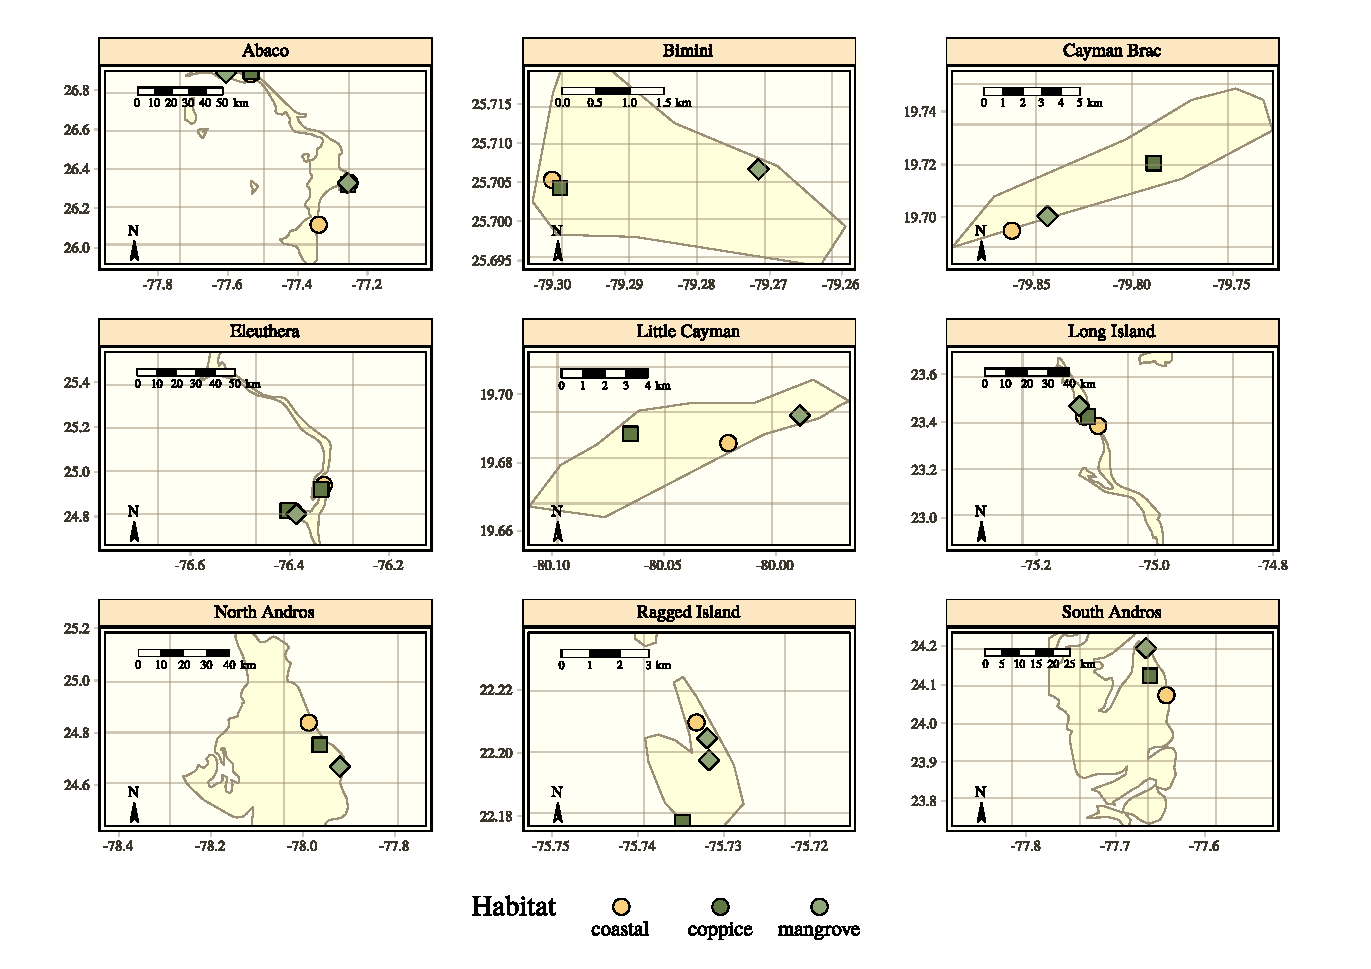
\includegraphics[width=\textwidth]{../maps/detailed_map.pdf}
	\caption{Map of the sampling sites and corresponding habitats across 9 islands of the West Indies.}
	\label{supfig:map}
\end{figure}

% Reflectance curves
\begin{figure}[H]
    \centering
	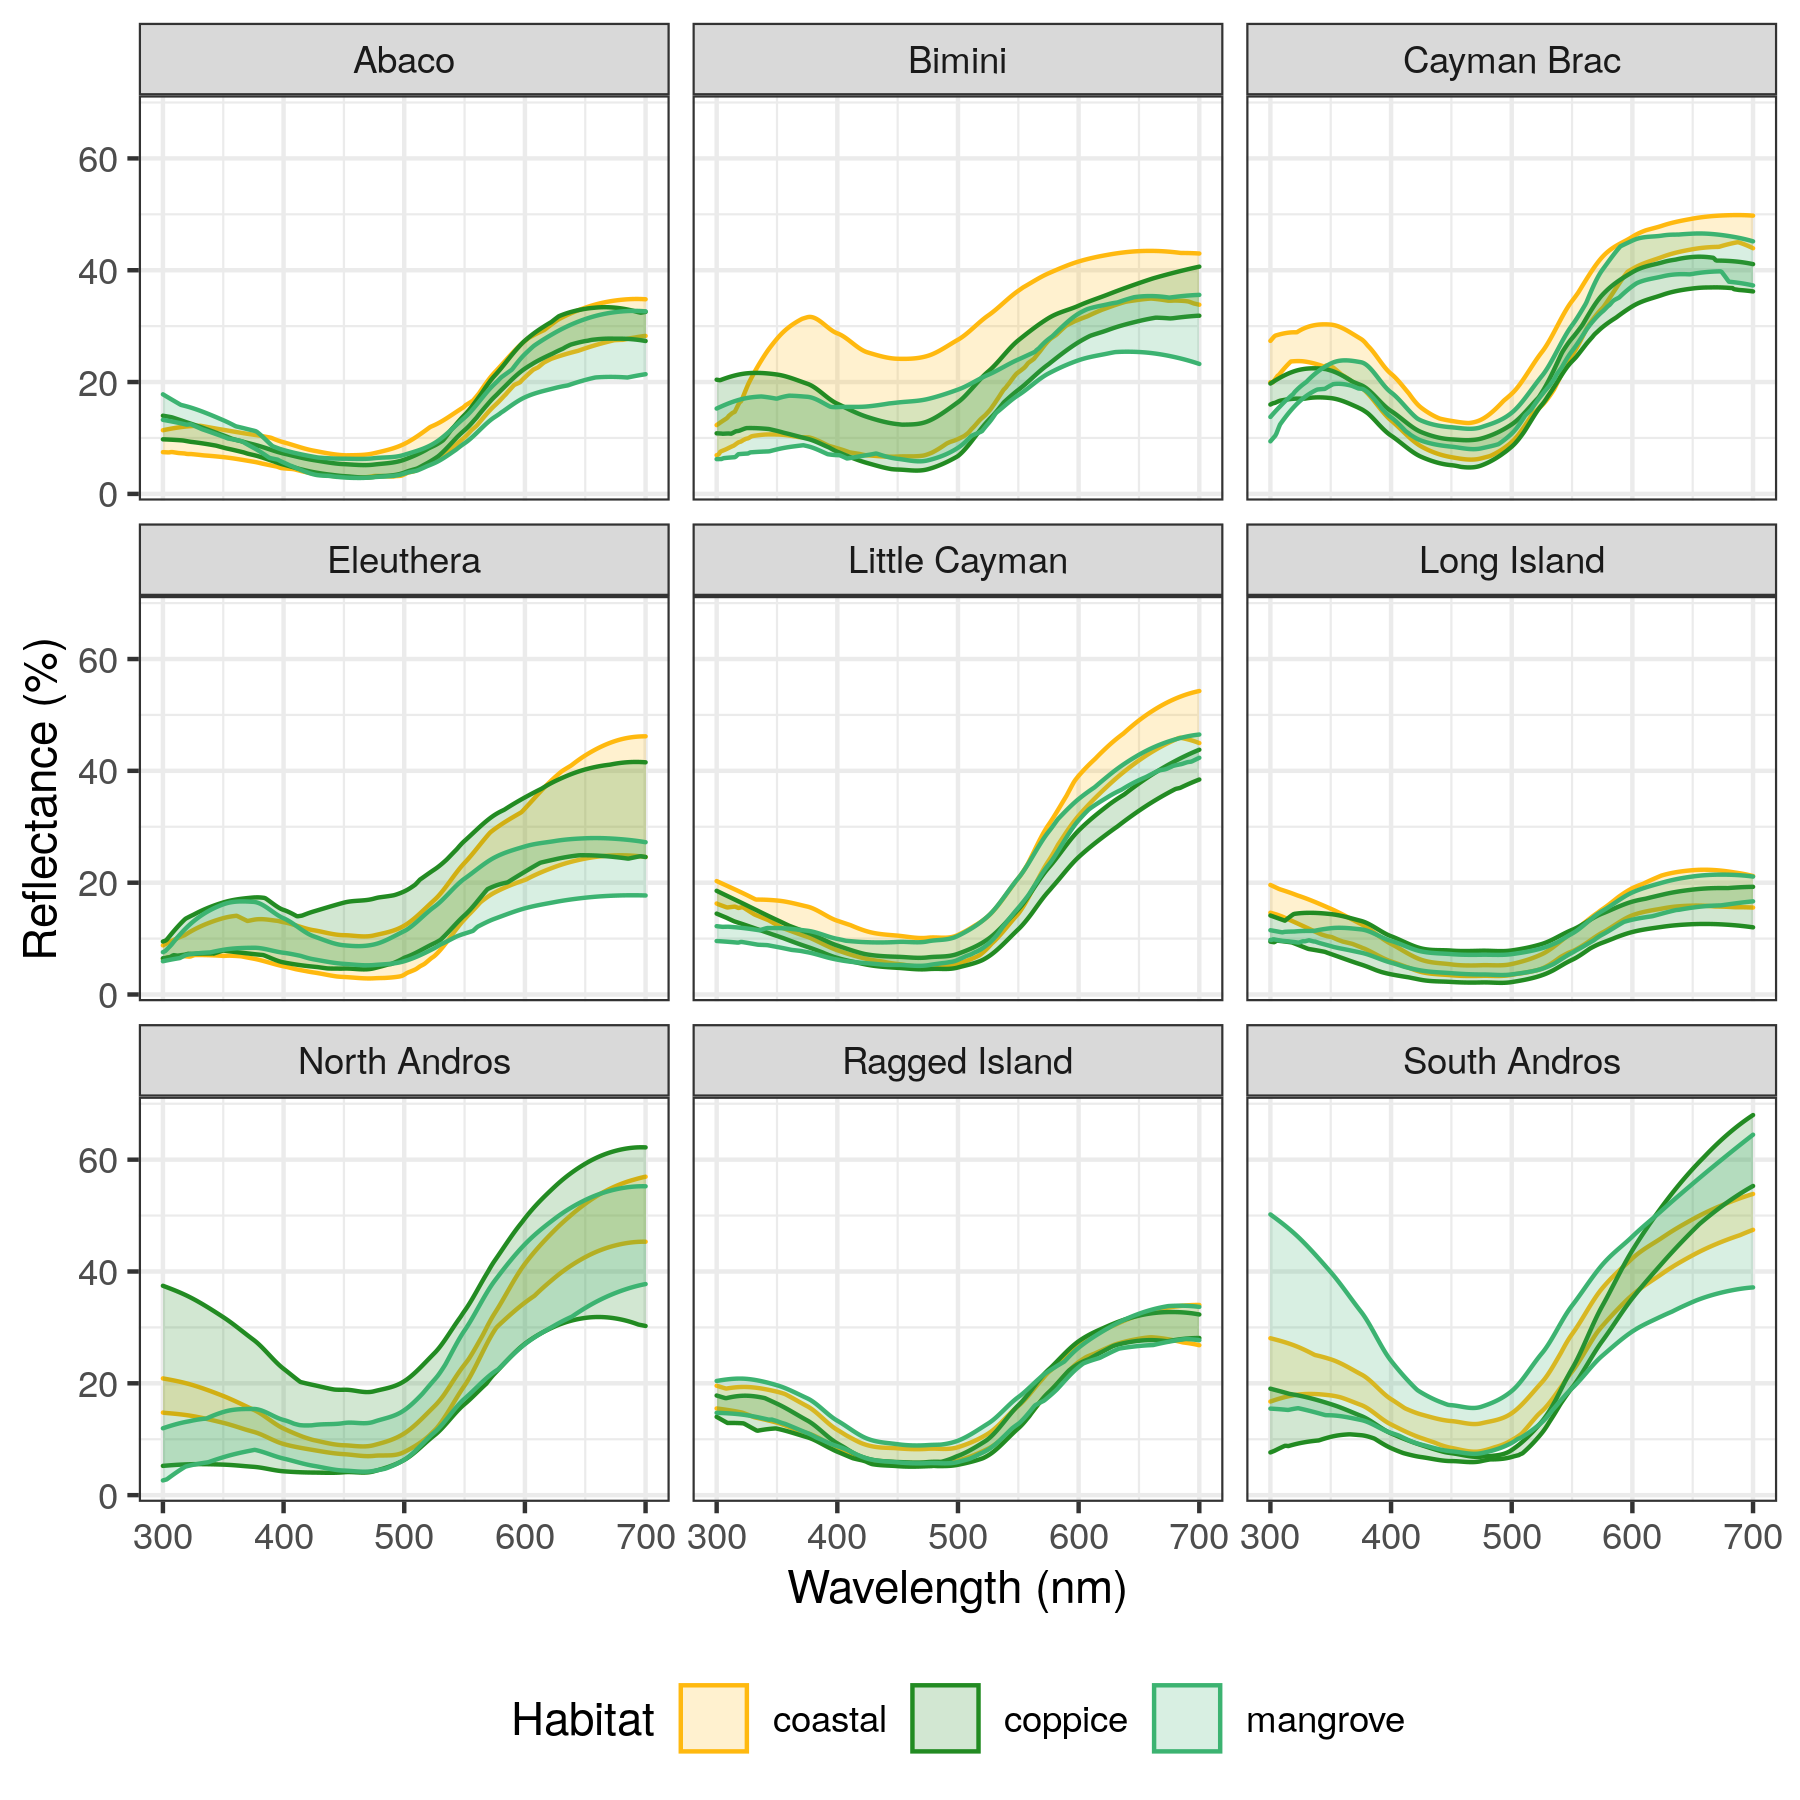
\includegraphics[width=\textwidth]{../analyses/02-reflectance/figure_reflectance.png}
	\caption{5-95th percentile distributions of lizard dewlap reflectance values (in \% of incoming light) across wavelengths for each island and each habitat.}
	\label{supfig:reflectance}
\end{figure}

% Classification accuracy of LDAs
\begin{figure}[H]
    \centering
	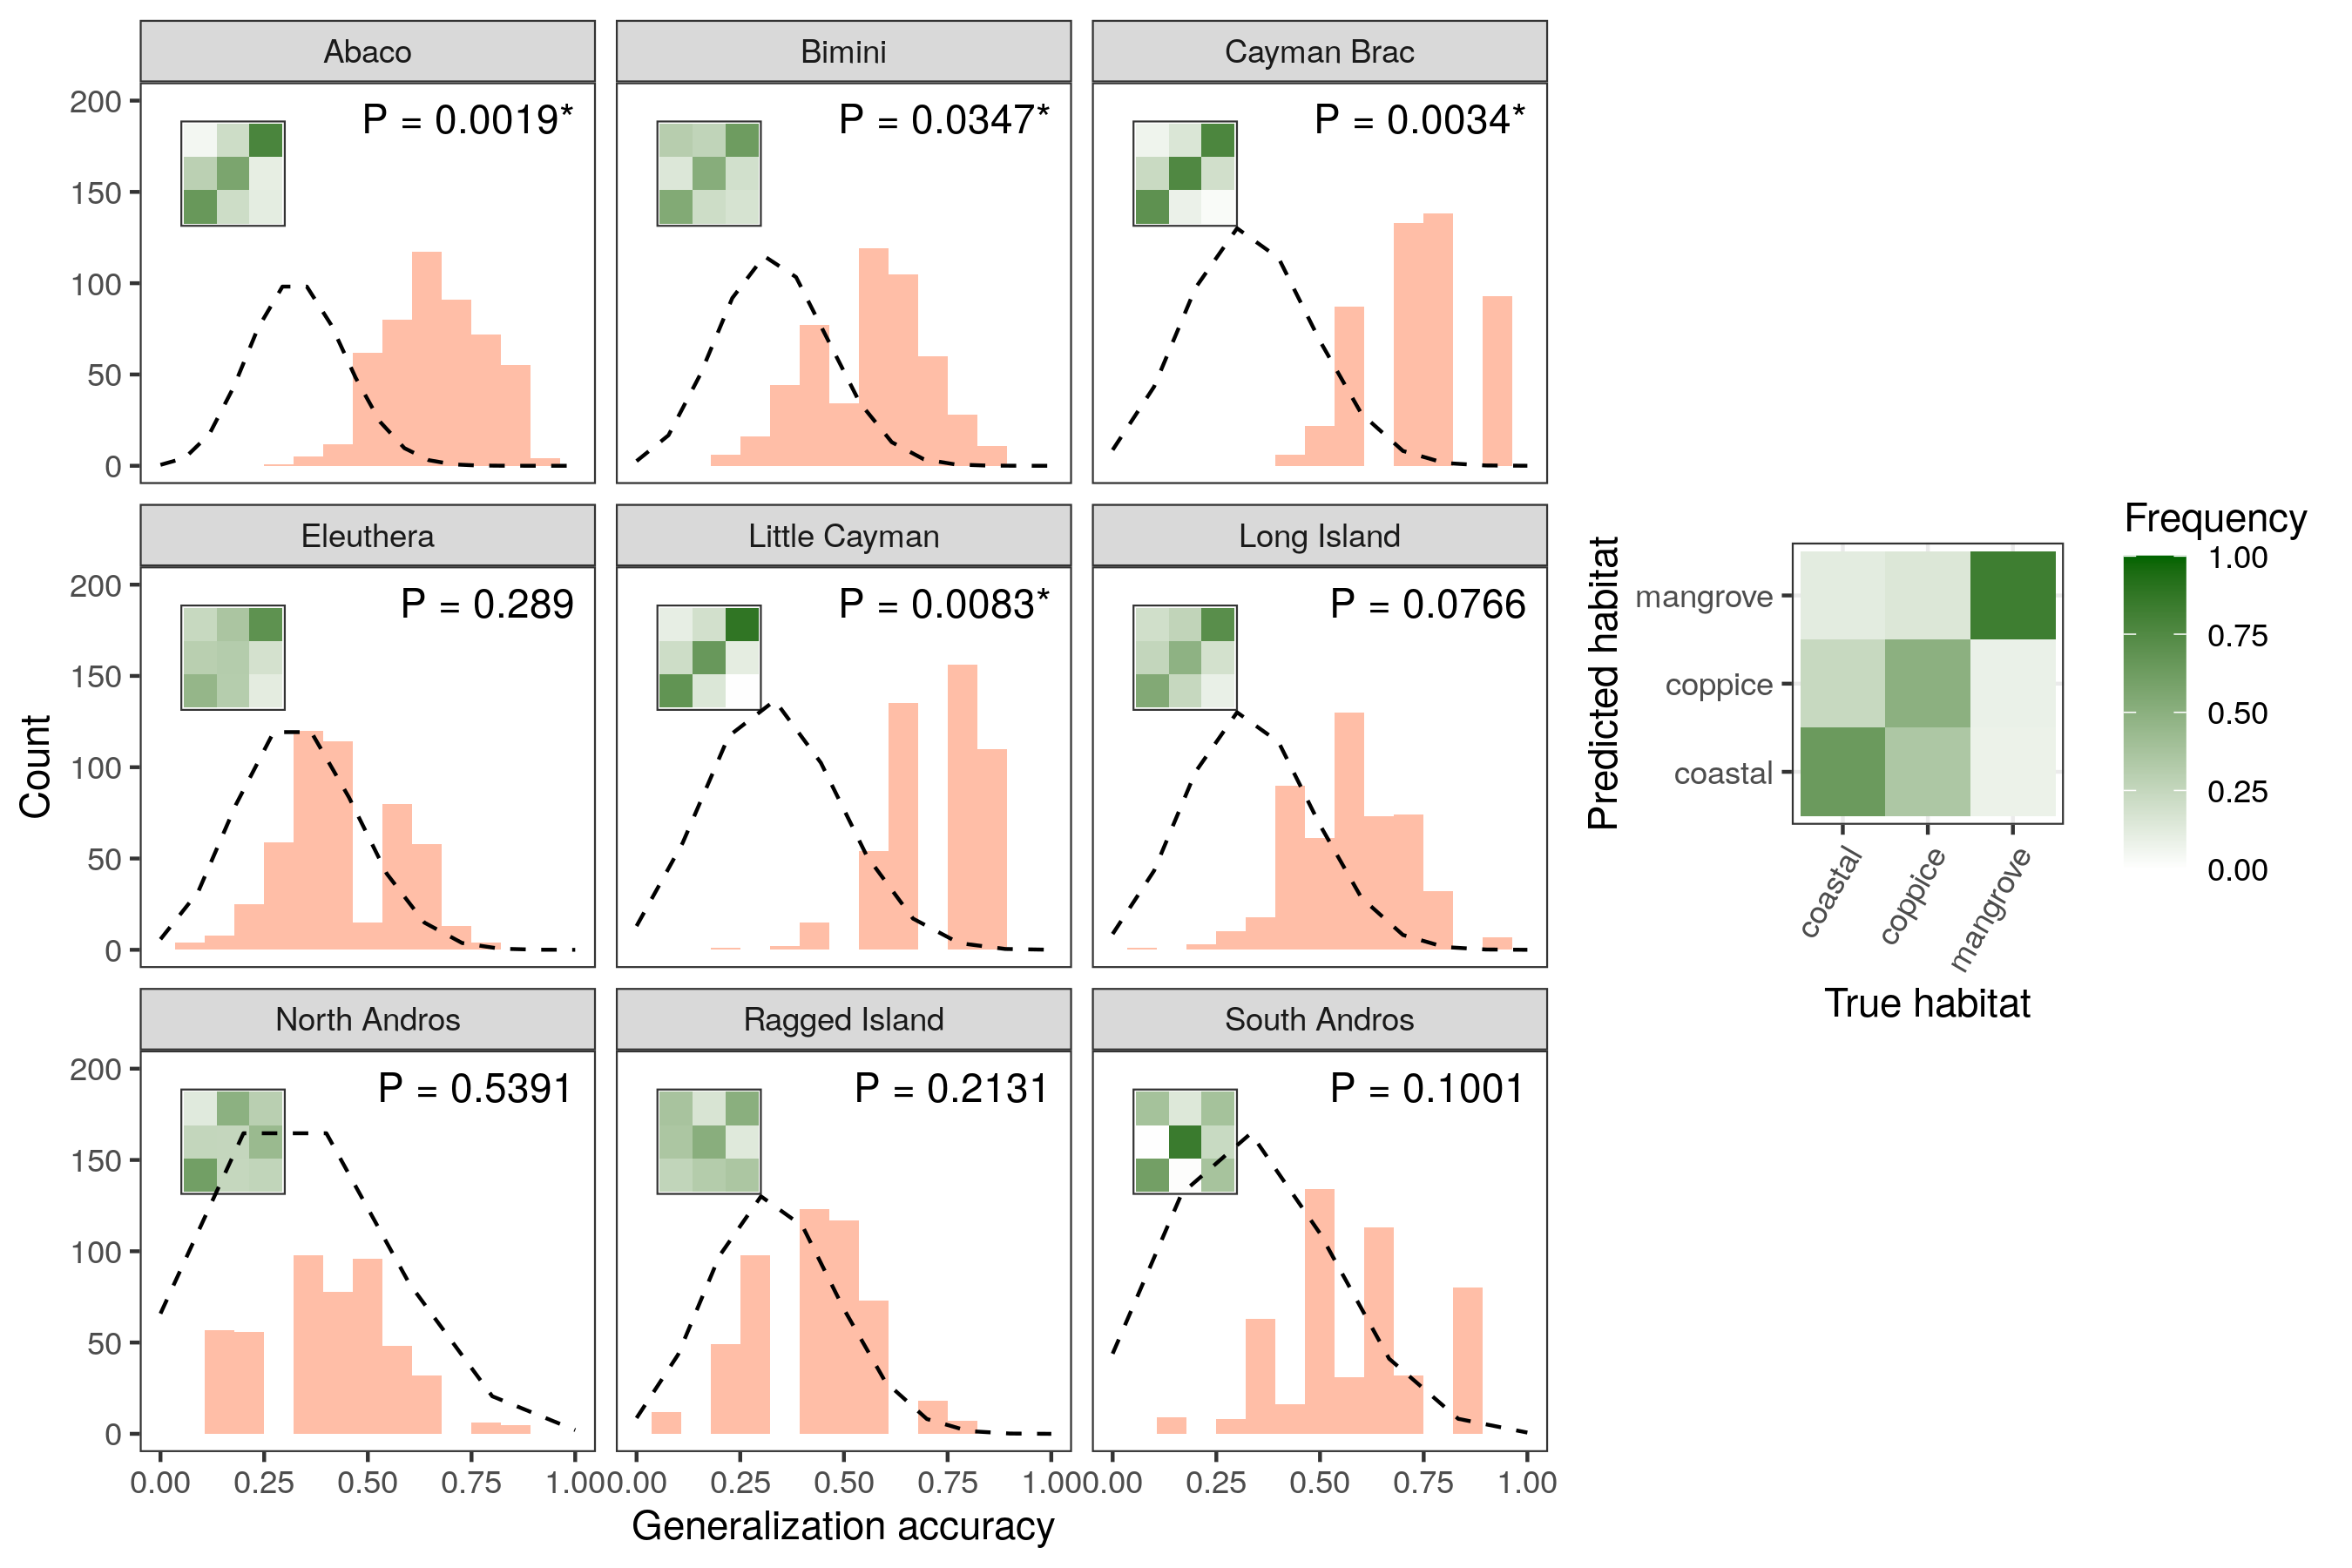
\includegraphics[width=\textwidth]{../analyses/04-machine learning/plots/classif_lda_pca.png}
	\caption{Distributions of classification accuracy across all LDA machines (100 replicates of 5 cross-validation bins each). The dashed line represents the density of a corresponding null binomial distribution, which would be expected under random guessing (testing sets with 20\% of the observations for each island and success probability of $1/3$). Inset plots show the corresponding average confusion matrices and represent the proportion of lizards from each habitat (columns) reassigned in each other habitat (rows), with an interpretation guide in the right panel. P-values indicate deviations of the mean classification accuracy to the expected null binomial distribution. *, P < 0.05}
	\label{supfig:classif_lda_pca}
\end{figure}

\begin{figure}[H]
    \centering
	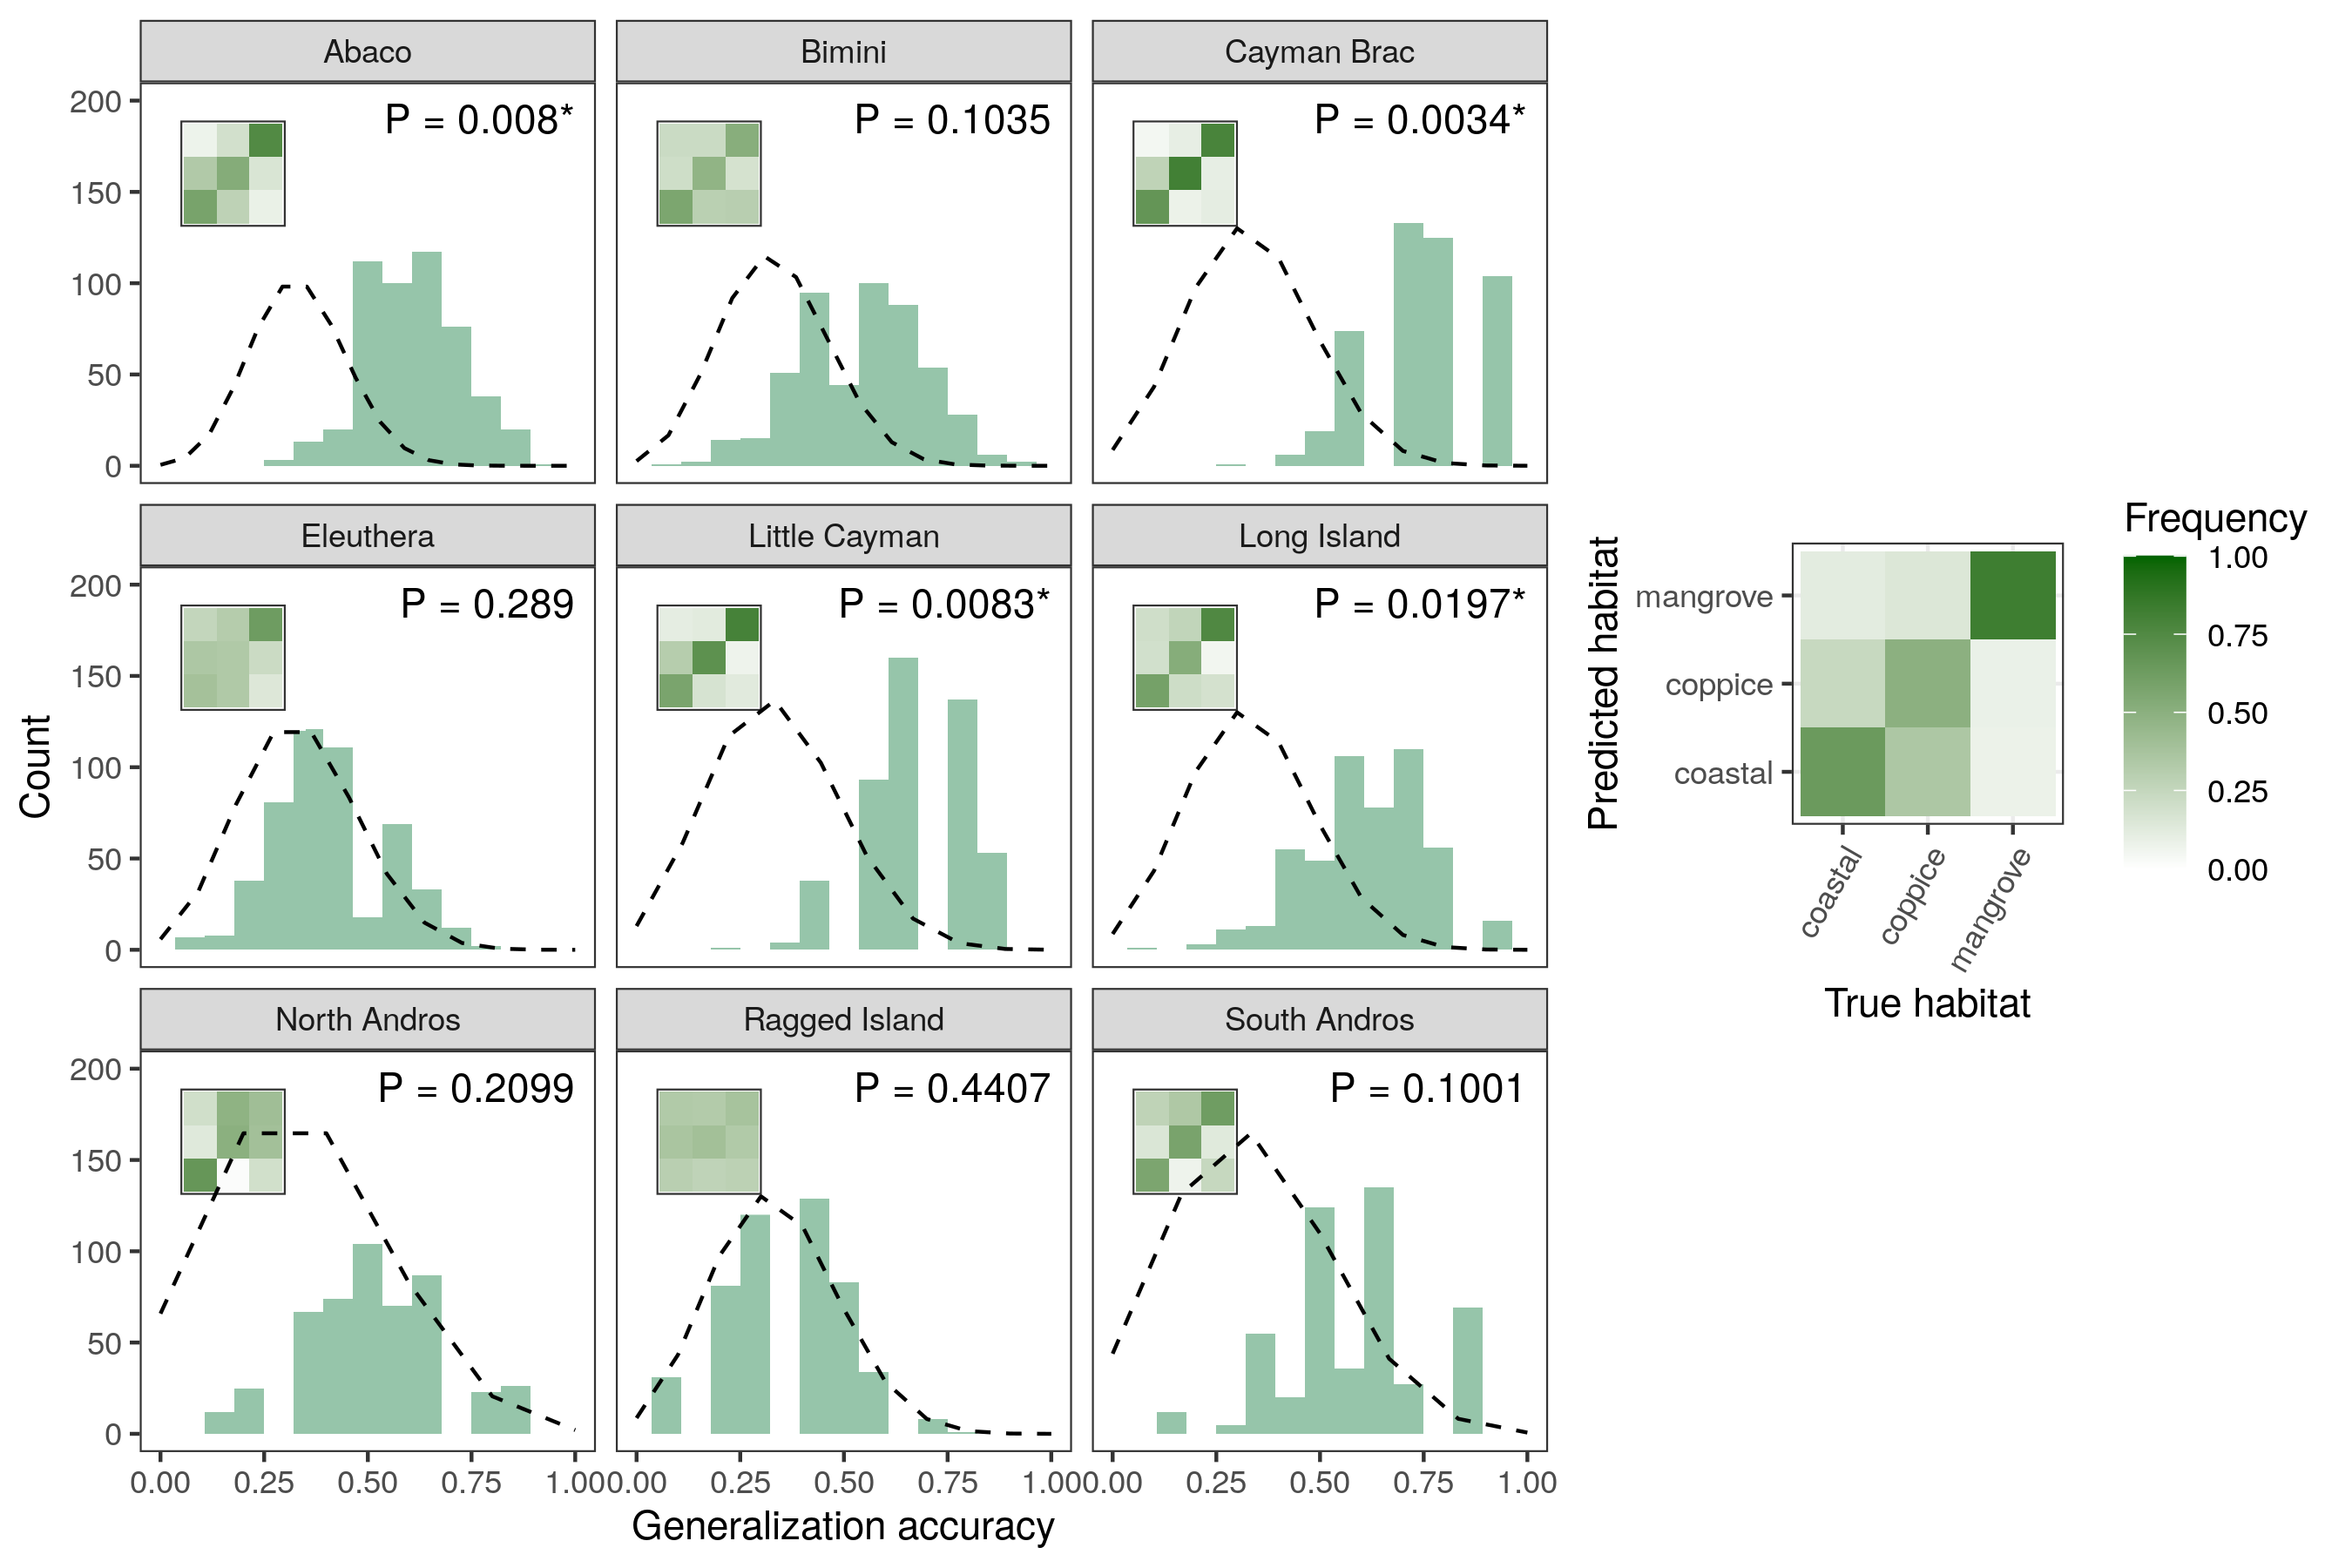
\includegraphics[width=\textwidth]{../analyses/04-machine learning/plots/classif_svm_refl.png}
	\caption{Distributions of classification accuracy across all SVM machines (100 replicates of 5 cross-validation bins each) trained directly on reflectance data from 300 to 700nm, at 50nm intervals. The dashed line represents the density of a corresponding null binomial distribution, which would be expected under random guessing (testing sets with 20\% of the observations for each island and success probability of $1/3$). Inset plots show the corresponding average confusion matrices and represent the proportion of lizards from each habitat (columns) reassigned in each other habitat (rows), with an interpretation guide in the right panel. P-values indicate deviations of the mean classification accuracy to the expected null binomial distribution. *, P < 0.05}
	\label{supfig:classif_svm_refl}
\end{figure}

\begin{figure}[H]
    \centering
	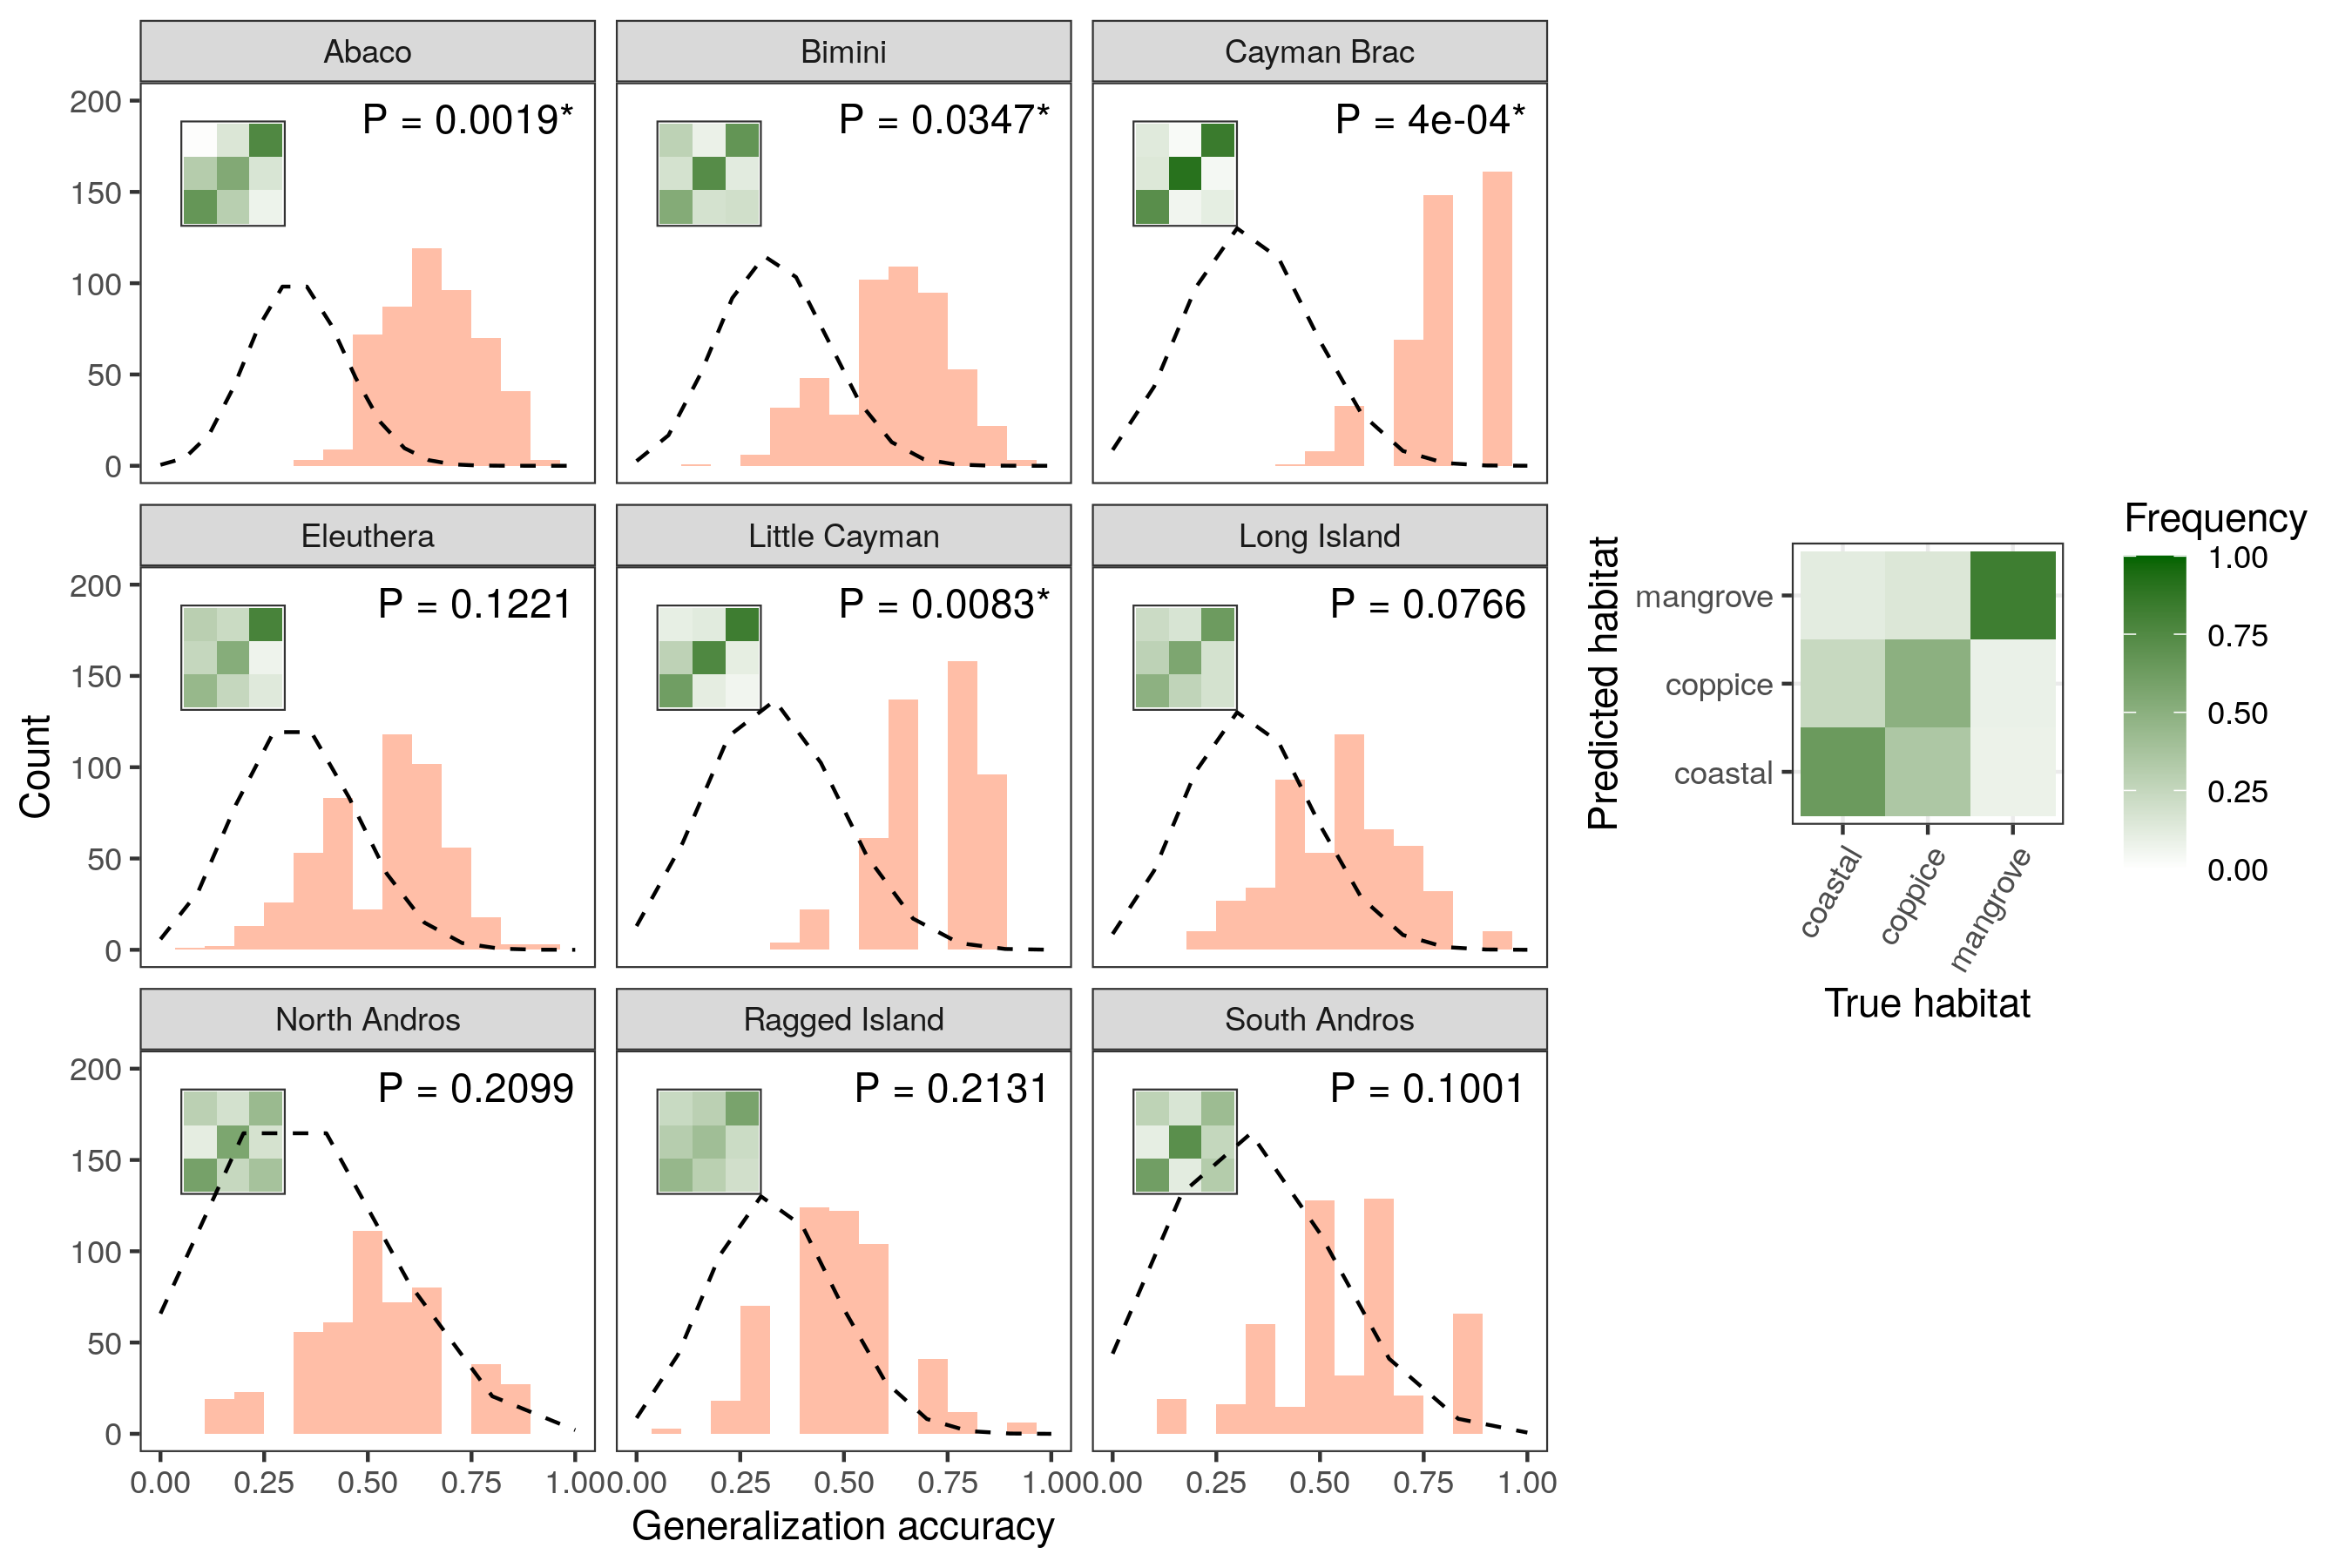
\includegraphics[width=\textwidth]{../analyses/04-machine learning/plots/classif_lda_refl.png}
	\caption{Distributions of classification accuracy across all LDA machines (100 replicates of 5 cross-validation bins each) trained directly on reflectance data from 300 to 700nm, at 50nm intervals. The dashed line represents the density of a corresponding null binomial distribution, which would be expected under random guessing (testing sets with 20\% of the observations for each island and success probability of $1/3$). Inset plots show the corresponding average confusion matrices and represent the proportion of lizards from each habitat (columns) reassigned in each other habitat (rows), with an interpretation guide in the right panel. P-values indicate deviations of the mean classification accuracy to the expected null binomial distribution. *, P < 0.05}
	\label{supfig:classif_lda_refl}
\end{figure}